\subsection{Online Clustering}

Detecting events in a stream of news articles will be achieved by using an online clustering approach. An event is described by the occurrence of multiple news articles to the same subject.  The events of interest for this application are the discovery of new topics and the extension of existing topics. Thus we define our two events as follows:

\begin{itemize}
    \item Topic added: A new cluster of news articles appears in the data stream.
    \item Topic extended: An existing topic is extended by additional news articles.
\end{itemize}

HDBSCAN will be applied as the clustering method, using the optimal settings as discovered in the previous evaluation. Additional preprocessing of news articles before clustering is going to be explored as part of evaluation as well and will be implemented accordingly for the online clustering.

Since HDBSCAN only supports static data sets, the clustering will be done in batches using a time based sliding window approach. Events are detected by comparing the resulting clusters with the previous ones.

\begin{figure}[h]
    \centering

    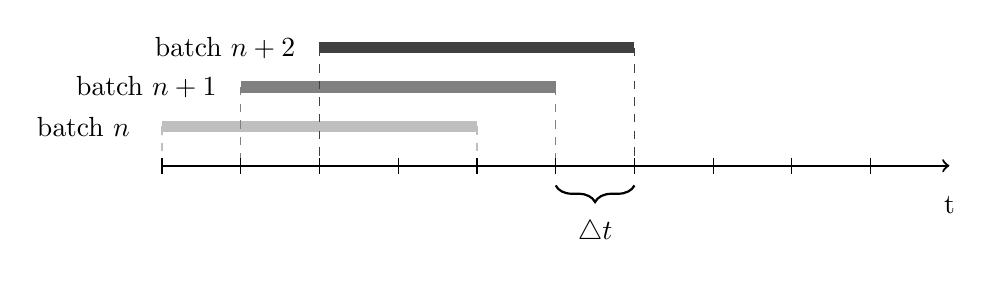
\begin{tikzpicture}[scale=1]

        \draw[lightgray, line width=4pt] (0,.5) -- (4,.5);
        \draw[lightgray, dashed] (0,.5) -- (0,0);
        \draw[lightgray, dashed] (4,.5) -- (4,0);
        \node[align=right] at (-1,.5) {batch $n$};

        \draw[gray, line width=4pt] (1,1) -- (5,1);
        \draw[gray, dashed] (1,1) -- (1,0);
        \draw[gray, dashed] (5,1) -- (5,0);
        \node[align=right] at (-.2,1) {batch $n + 1$};

        \draw[darkgray, line width=4pt] (2,1.5) -- (6,1.5);
        \draw[darkgray, dashed] (2,1.5) -- (2,0);
        \draw[darkgray, dashed] (6,1.5) -- (6,0);
        \node[align=right] at (0.8,1.5) {batch $n + 2$};

        \node[align=center] at (5.5,-0.85) {$\triangle t$};
        \node[align=center] at (10,-0.5) {t};

        \draw [thick,->] (0,0) -- (10,0);
        \foreach \x in {0,...,9} \draw (\x,0.1) -- (\x,-0.1);

        \draw [thick,decorate,decoration={brace,amplitude=6pt,raise=0pt,mirror}] (5,-0.25) -- (6,-0.25);

        \end{tikzpicture}

    \caption{Timeline showing the sliding window approach}
    \label{fig:timeline}
\end{figure}

\paragraph{Finding pairs clusters}
Thus we define our two events as follows:
To be able to compare clusters of different batches with each other, we have to find pairs of clusters between batches, which describe the same topic. This is done by applying the same assumptions as for the scoring function used in the evaluation. Therefore clusters are paired based on their similarity calculated with the Jaccard index as shown in equation \ref{equ:similarity}. If the similarity is above a certain threshold, both clusters are seen as describing the same topic.

\paragraph{Sliding window}

An important consideration for determining existing or new clusters is the overlap of samples between batches. If the overlap is too small, similar clusters will no longer be detected as such, which would result in an increasingly high error rate. Finding optimal values for the step size between batches and the number of samples for each batch is therefore essential for our online clustering approach.

\subsubsection{Implementation}

The online clustering implemented for this thesis does not operate in a true online setting, but rather it takes our existing test data and simulates a data stream over time. The simulated approach allows us to directly compare the resulting events with the ground truth and thus evaluate different settings. The implementation is done with Python and the application provides a command line interface to run the simulation with different parameters such as the start date, number of days to run and the batch size.

\paragraph{Comparing clusters}
To detect events between batches of clusterings,
we have find pairs of clusters describing the same topic.
This problem is solved in the evaluation framework as part of the scoring function,
by calculating the similarity for each possible cluster pair.
The resulting time complexity is $O(n^2)$, which we deemed acceptable for the static evaluation.
However in a dynamic setting such as the online clustering, performance is an important factor,
since it restricts the lengths of the time delta between batches and the overall batch size.
Thus we decided to use Locality-Sensitive Hashing (LSH)\cite{alex2015practical} to find similar clusters.
This reduces the time complexity to $O(log(n))$.
The implementation for LSH is provided by the datasketch library\cite{eric_zhu_2017_290602}.
% TODO explain LSH?

\paragraph{Detecting Events}
Once we have found pairs of clusters, which represent the same topic, detecting events becomes trivial.
For each pair we look for news articles, which are only present in the new cluster.
These articles are then summarized in the event \textit{topic extended} for a specific topic.
Clusters from the new batch without a matching cluster from the previous batch
are seen as new topics and represented by the event \textit{topic added}.

% TODO clarify event vs topic vs story and be consistent with the usages!